\documentclass[a4paper,12pt]{article}

\usepackage[
    left=2cm,
    right=2cm,
    top=3cm,
    bottom=3cm
]{geometry}

\usepackage[utf8]{inputenc}
\usepackage[czech]{babel}
\usepackage[T1]{fontenc}
\usepackage{graphicx}
\usepackage{array}
\usepackage{booktabs}
\usepackage{tabularx}
\usepackage{makecell}
\usepackage{float}
\usepackage{newunicodechar}
\usepackage{url}
\usepackage{siunitx}
\usepackage{listings}
\usepackage{gensymb}
\usepackage{xcolor}
\usepackage{diagbox}
\usepackage{hyperref}
\usepackage{tikz}
\usepackage{pgfplots}
\pgfplotsset{compat=1.18}

\usepackage{fancyhdr}
\pagestyle{fancy}

\fancyhf{}
\fancyhead[L]{SME -- Lab 2: Měření teploty termočlánky}
\fancyhead[R]{Pavel Pernička}
\fancyfoot[C]{\thepage}

\fancypagestyle{firstpage}{
    \fancyhf{}
    \renewcommand{\headrulewidth}{0pt}
    \renewcommand{\footrulewidth}{0pt}
    \fancyfoot[C]{\thepage}
}

\definecolor{myblue}{RGB}{111,0,248}
\newcommand{\colorcircle}[1]{%
  \tikz[baseline=-0.6ex]\draw[fill=#1,draw=none] (0,0) circle (1.5ex);%
}
\newcommand{\unitC}{\,^\circ\mathrm{C}}
\newcommand{\unitV}{\,\mathrm{V}}
\newcommand{\unitA}{\,\mathrm{A}}
\newcommand{\units}{\,\mathrm{s}}
\newcommand{\unitmin}{\,\mathrm{min}}

\newcommand{\centered}[1]{\begin{tabular}{l} #1 \end{tabular}}

\addto\captionsczech{\renewcommand{\refname}{Seznam použité literatury}}
\addto\captionsczech{\renewcommand{\figurename}{\textbf{Obrázek}}}
\addto\captionsczech{\renewcommand{\tablename}{\textbf{Tabulka}}}
\renewcommand{\lstlistingname}{\textbf{Kód}}

\lstset{
    language=Python,
    basicstyle=\ttfamily\footnotesize,
    keywordstyle=\color{blue},
    commentstyle=\color{gray},
    stringstyle=\color{red},
    numbers=left,
    numberstyle=\tiny\color{gray},
    stepnumber=1,
    breaklines=true,
    frame=single
}

\begin{document}
\thispagestyle{firstpage}

\vspace*{\fill}
\begin{center}
\renewcommand{\arraystretch}{1.75}

\begin{tabularx}{\textwidth}{|X|X|X|}
    \hline
    \multicolumn{1}{|c|}{\rule{0pt}{2.25cm} 
\includegraphics[height=2cm]{img/ctu_logo.png}}
    & \multicolumn{2}{c|}{\makecell{\textbf{KATEDRA MĚŘENÍ}}} \\
    \hline
    \multicolumn{3}{|c|}{\Large \textbf{\centered{Senzory a měření}}} \\
    \hline
    \multicolumn{2}{|X}{\small{Jméno} \newline \textbf{Pavel Pernička}}
    & \multicolumn{1}{|X|}{\small{Datum měření} \newline \textbf{18.3.2026}} \\
    \hline
    {\small{Semestr} \newline \textbf{Letní 2026}}
    & {\small{Ročník} \newline \textbf{2.}}
    & {\small{Datum odevzdání} \newline \textbf{25.3.2026}} \\
    \hline
    \multicolumn{3}{|c|}{\rule{0pt}{1cm}} \\
    \hline
    \multicolumn{1}{|X|}{\small{Číslo úlohy \newline \textbf{2}}}
    & \multicolumn{2}{|p{9cm}|}{\small{Název úlohy \newline \textbf{Měření teploty termočlánky}}} \\
    \hline
\end{tabularx}

\end{center}
\vspace*{\fill}

\newpage
\pagestyle{fancy}
\section{Domácí příprava}
\begin{itemize}
  \item Jaká je teplota srovnávacího spoje („studeného konce“), na kterou koriguje kompenzační obvod? Dá se to zjistit jednoduchým měřením?
    \begin{itemize}
      \item V našem případě se jedná o pokojovou teplotu, protože srovnávací spoj nijak nezahříváme a je dostatečně vzdálen od měřicího konce. Měříme pomocí teploměru, který je součástí setu.
    \end{itemize}
  \item Čemu se rovná vstupní a výstupní odpor invertujícího a neinvertujícího zesilovače s ideálním operačním zesilovačem?
    \begin{itemize}
      \item Vstupní odpor invertujícího zesilovače je roven odporu $R_1$ na obrázku. Výstupní odpor je v ideálním případě nulový.
      \item Vstupní odpor neinvertujícího zesilovače v případě na obrázku je roven odporu rezistoru paralelně se vstupem. Tedy $100\ k\Omega$
\begin{figure}[H]
\centering
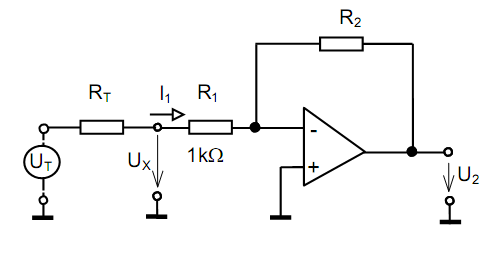
\includegraphics[width=0.5\textwidth]{img/inverting.png}
\caption{Invertující OZ}
\label{fig:char}
\end{figure}

\begin{figure}[H]
\centering
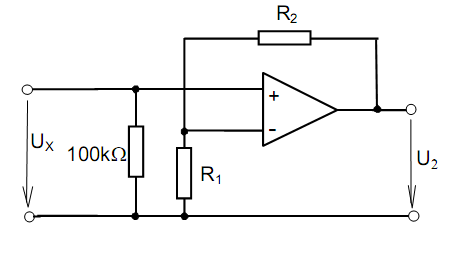
\includegraphics[width=0.5\textwidth]{img/noninverting.png}
\caption{Neinvertující OZ}
\label{fig:char}
\end{figure}


    \end{itemize}
  \item Jak lze korigovat vstupní napěťovou nesymetrii zesilovače?
    \begin{itemize}
      \item Buď pomocí odporového děliče přivedeme na vstup OZ kompenzačnínapětí, nebo napěťovou nesymetrii softwarově odečteme z naměřeného napětí.
    \end{itemize}
  \item Je vhodné použít termočlánek pro měření pokojové teploty? Vysvětlete.
    \begin{itemize}
      \item Ne, pracuje totiž na principu Seebackova jevu a aby vzniklo nějaké napětí, je potřeba teplotní gradient v materiálu termočlánku. Pro měření pokojové teploty bychom museli např. dostatečně ochlazovat srovnávací spoj na známou teplotu.
    \end{itemize}
\end{itemize}

\section{Měření}
Pro měření používáme chromel-alumelový termočnánek s konstantou $K_t = 0,0408\ mV\cdot K^{-1}$ v~našem měřeném rozsahu.
\subsection{Teplota v kalibrační pícce bez OZ}
Při srovnávací teplotě $T_S = 19\ \degree C$ jsme naměřili následující hodnoty:
\begin{table}[H]
\centering
\begin{tabular}{|l|c|c|}
\hline
 & Ruční multimetr & Stolní multimetr \\ \hline
Bez kompenzace & $3,1\ \mathrm{mV}$ & $3,111\ \mathrm{mV}$ \\ \hline
S kompenzací   & $3,9\ \mathrm{mV}$ & $3,941\ \mathrm{mV}$ \\ \hline
\end{tabular}
\caption{Naměřená napětí bez OZ}
\end{table}
Výpočet teploty:
$$
T = \frac{U_n}{K_t} + T_S
$$
($T_S$ je v případě použití kompenzačního obvodu rovna nule)

\begin{table}[H]
\centering
\begin{tabular}{|l|c|c|}
\hline
 & Ruční multimetr & Stolní multimetr \\ \hline
Bez kompenzace & $95{,}0\ ^\circ C$ & $95{,}3\ ^\circ C$ \\ \hline
S kompenzací   & $94{,}6\ ^\circ C$ & $96{,}6\ ^\circ C$ \\ \hline
\end{tabular}
\caption{Vypočítané teploty bez OZ}
\end{table}

\subsection{Nejistota měření}
\begin{itemize}
  \item Přesnost multimetru EX-350: $\pm(0,7\% + 5\ digit)$ v range do $40\ mV$
  \item Přesnost stolního voltmetru Agilent 34401A: $\pm(0,00003\% + 0,003\ mV)$
\end{itemize}

\subsection{Rozšířená nejistota měření napětí termočlánku}
\subsection{Nejistota měření}

Koeficient rozšíření:
$$
k_r = 2
$$

Standardní nejistota typu B:
$$
u_B = \frac{\Delta U}{\sqrt{3}}
$$

\subsubsection*{Ruční multimetr EX-350}
$$
\Delta U_r = 0{,}007 \cdot 3{,}9 + 0{,}05 = 0{,}0773\ \mathrm{mV}
$$

$$
u_{B,r} = \frac{0{,}0773}{\sqrt{3}} \approx 0{,}0446\ \mathrm{mV}
$$

$$
u_r = 2u_{B,r} \approx 0{,}089\ \mathrm{mV}
$$

\subsubsection*{Stolní multimetr Agilent 34401A}
$$
\Delta U_s = 0{,}00003 \cdot 3{,}941 + 0{,}003 \approx 0{,}00312\ \mathrm{mV}
$$

$$
u_{B,s} = \frac{0{,}00312}{\sqrt{3}} \approx 0{,}00180\ \mathrm{mV}
$$

$$
u_s = 2u_{B,s} \approx 0{,}0036\ \mathrm{mV}
$$
\subsection{Teplota v kalibrační pícce s OZ}
Operační zesilovač zapojíme jako neinvertující podle následujícího schématu, kde $R_1=1\ k\Omega$ a~$R_2 = 100\ k\Omega$. Zesílení tedy bude $z = (1+\frac{R_2}{R_1}) = 101$ krát.

\begin{figure}[H]
\centering

\includegraphics[width=0.5\textwidth]{img/schematic.png}
\caption{Zapojení OZ}
\label{fig:char}
\end{figure}

\begin{table}[H]
\centering
\begin{tabular}{|l|c|c|}
\hline
 & Ruční multimetr & Stolní multimetr \\ \hline
Naměřeno & $0{,}3218\ \mathrm{V}$ & $0{,}3225\ \mathrm{V}$ \\ \hline
Pův. napětí & $3{,}186\ \mathrm{mV}$ & $3{,}193\ \mathrm{mV}$ \\ \hline
Teplota & $97{,}1\ ^\circ C$ & $97{,}3\ ^\circ C$ \\ \hline
\end{tabular}
\caption{Naměřené a vypočtené hodnoty s OZ}
\end{table}

\subsection{Vstupní napěťová nesymetrie OZ}
\subsubsection*{Komutace výstupu termočlánku}
Uděláme 2 měřením kdy mezi nimi prohodíme polaritu termočlánku. Napěťovou nesymetrii pak vypočítáme jako:

$$
U_1 = z(U_{term.} + U_{offset})
$$
$$
U_2 = z(-U_{term.} + U_{offset})
$$
$$
U_1 + U_2 = 2 z U_{offset}
$$
$$
U_{offset} = \frac{U_1+U_2}{2z}
$$

Naměřili jsme $U_1 = 0,31924\ V$ a $U_2 = 0,31530\ V$. Tedy $U_{offset} = 19,6\ \mu V$.
\subsubsection*{Zkratovaný vstup OZ}
Offset vypočítáme jako:
$$
U_{offset} = \frac{U_1}{z}
$$

Naměřili jsme $U_1 = 2,127\ mV$, offset je tedy $U_{offset} = 21,27\ \mu V$

Obě naměřené hodnoty vypadají reálně a jsou dokonce pod typickým rozmezím z datasheetu.

\subsection{Teplota v kalibrační pícce pomocí USB modulu}
Naměřená data jsou na obrázku.

\begin{figure}[H]
\centering
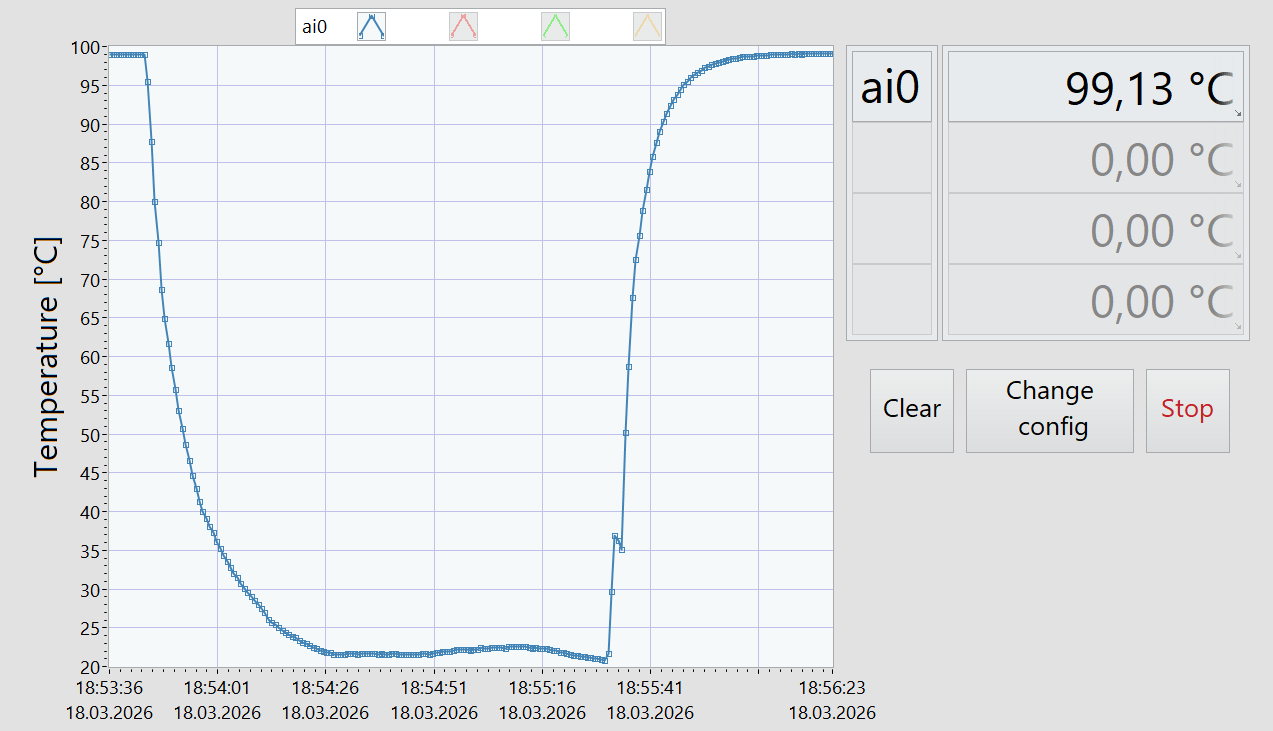
\includegraphics[width=0.9\textwidth]{img/usb_temperature.png}
\caption{Teplota naměřená pomocí USB modulu}
\label{fig:char}
\end{figure}

\subsection{Porovnání}
Teploty naměřené bez operačního zesilovače jsou mezi sebou konzistentní, protože byly měřeny v jedné poleze termočlánku v peci. Z nich by měla být nejpřesnější hodnota naměřená stolním voltmetrem a s kompenzací. 

Hodnoty naměřené s použitím OZ jsou oproti těm předchozím posunuté, zejména protože jsme senzor mezi měřeními z pícky vytáhli a následně vložili v jiné poloze. 

\end{document}
